\documentclass{article}\usepackage[]{graphicx}\usepackage[]{xcolor}
% maxwidth is the original width if it is less than linewidth
% otherwise use linewidth (to make sure the graphics do not exceed the margin)
\makeatletter
\def\maxwidth{ %
  \ifdim\Gin@nat@width>\linewidth
    \linewidth
  \else
    \Gin@nat@width
  \fi
}
\makeatother

\definecolor{fgcolor}{rgb}{0.345, 0.345, 0.345}
\newcommand{\hlnum}[1]{\textcolor[rgb]{0.686,0.059,0.569}{#1}}%
\newcommand{\hlstr}[1]{\textcolor[rgb]{0.192,0.494,0.8}{#1}}%
\newcommand{\hlcom}[1]{\textcolor[rgb]{0.678,0.584,0.686}{\textit{#1}}}%
\newcommand{\hlopt}[1]{\textcolor[rgb]{0,0,0}{#1}}%
\newcommand{\hlstd}[1]{\textcolor[rgb]{0.345,0.345,0.345}{#1}}%
\newcommand{\hlkwa}[1]{\textcolor[rgb]{0.161,0.373,0.58}{\textbf{#1}}}%
\newcommand{\hlkwb}[1]{\textcolor[rgb]{0.69,0.353,0.396}{#1}}%
\newcommand{\hlkwc}[1]{\textcolor[rgb]{0.333,0.667,0.333}{#1}}%
\newcommand{\hlkwd}[1]{\textcolor[rgb]{0.737,0.353,0.396}{\textbf{#1}}}%
\let\hlipl\hlkwb

\usepackage{framed}
\makeatletter
\newenvironment{kframe}{%
 \def\at@end@of@kframe{}%
 \ifinner\ifhmode%
  \def\at@end@of@kframe{\end{minipage}}%
  \begin{minipage}{\columnwidth}%
 \fi\fi%
 \def\FrameCommand##1{\hskip\@totalleftmargin \hskip-\fboxsep
 \colorbox{shadecolor}{##1}\hskip-\fboxsep
     % There is no \\@totalrightmargin, so:
     \hskip-\linewidth \hskip-\@totalleftmargin \hskip\columnwidth}%
 \MakeFramed {\advance\hsize-\width
   \@totalleftmargin\z@ \linewidth\hsize
   \@setminipage}}%
 {\par\unskip\endMakeFramed%
 \at@end@of@kframe}
\makeatother

\definecolor{shadecolor}{rgb}{.97, .97, .97}
\definecolor{messagecolor}{rgb}{0, 0, 0}
\definecolor{warningcolor}{rgb}{1, 0, 1}
\definecolor{errorcolor}{rgb}{1, 0, 0}
\newenvironment{knitrout}{}{} % an empty environment to be redefined in TeX

\usepackage{alltt}
\usepackage[utf8]{inputenc}
\usepackage{amsfonts}
\usepackage{tgpagella}
\usepackage{graphicx} % Required for inserting images
\usepackage{polski}
\renewcommand*{\figurename}{Rysunek}
\usepackage{nicefrac, xfrac}
\usepackage[margin=1in]{geometry}
\usepackage{hyperref}
\usepackage{xcolor}
\usepackage{amssymb}
\usepackage[bottom]{footmisc}
\usepackage{float}
\IfFileExists{upquote.sty}{\usepackage{upquote}}{}
\begin{document}



\section{Odsetek naprawianych marek pojazdów}
%Odsetek naprawianych marek pojazdów.

Przeprowadzono analizę, aby sprawdzić jakich marek pojazdy najczęściej pojawiają się w warsztacie do naprawy. 



Można przedstawić procentowy udział marek pojazdów klientów salonu, zaczynając od najczęściej się pojawiającej:

\begin{verbatim}
1. Volkswagen: 14.22%
2. Opel: 11.61%
3. Ford: 8.77%
4. Renault: 6.16%
5. Audi: 6.16%
6. Hyundai: 4.98%
7. Skoda: 4.98%
8. Fiat: 4.74%
9. Bajaj: 4.27%
10. Mercedes-Benz: 3.79%
11. BMW: 3.08%
12. Citroen: 3.08%
13. SEAT: 3.08%
14. Honda: 2.61%
15. Kia: 2.37%
16. Suzuki: 2.37%
17. Nissan: 2.13%
18. Peugeot: 2.13%
19. Mazda: 1.9%
20. Yamaha: 1.66%
21. Hero: 1.42%
22. Toyota: 1.42%
23. TVS: 1.42%
24. Volvo: 1.18%
25. Mitsubishi: 0.95%
26. Porsche: 0.71%
27. Dacia: 0.71%
28. Royal: 0.47%
29. SsangYong: 0.24%
30. MINI: 0.24%
31. Dodge: 0.24%
32. Vespa: 0.24%
33. Microcar: 0.24%
34. Jeep: 0.24%
35. Chevrolet: 0.24%
36. Mahindra: 0.24%
37. Jaguar: 0.24%
\end{verbatim}

{\color{red} PROCENTY ZNAK}

Jak widać, najpopularniejsze są pojazdy marki Volkswagen. Pojazdy tej marki stanowią 14.22 wszystkich. \\

Najmniej popularne są marki MINI, Dodge, Vespa, Microcar, Jeep, Chevrolet, Mahindra, Jaguar i SsangYong. Każdą z nich reprezentowało 0.24 pojazdów, które się pojawiły w warsztacie.

Sprawdzono także, jak prezentowałyby się rozkład marek, gdyby brano pod uwagę jedynie samochody



Można przedstawić ranking marek, zaczynając od najczęściej się pojawiającej:

\begin{verbatim}
1. Volkswagen: 16.13%
2. Opel: 13.17%
3. Ford: 9.95%
4. Audi: 6.99%
5. Renault: 6.99%
6. Skoda: 5.65%
7. Hyundai: 5.65%
8. Fiat: 5.38%
9. Mercedes-Benz: 4.3%
10. BMW: 3.49%
11. SEAT: 3.49%
12. Citroen: 3.49%
13. Kia: 2.69%
14. Nissan: 2.42%
15. Peugeot: 2.42%
16. Mazda: 2.15%
17. Suzuki: 1.88%
18. Toyota: 1.61%
19. Volvo: 1.34%
20. Mitsubishi: 1.08%
21. Dacia: 0.81%
22. Porsche: 0.81%
23. Honda: 0.81%
24. Chevrolet: 0.27%
25. MINI: 0.27%
26. Jeep: 0.27%
27. SsangYong: 0.27%
28. Microcar: 0.27%
29. Jaguar: 0.27%
30. Dodge: 0.27%
\end{verbatim}

Wśród aut prym wiedzie Volkswagen, reprezentując  16.13 naprawianych samochodów. \\

Najmniej było samochodów marek MINI, Jeep, SsangYong, Microcar, Jaguar, Dodge i Chevrolet. Było ich 0.27 dla każdej. \\

{\color{red} Coś o tym, czy się zgadza z pojazdami}

Pozostały do sprawdzenia motory.



Udział procentowy poszczególnych marek wśród nich prezentuje się następująco:

\begin{verbatim}
1. Bajaj: 36%
2. Honda: 16%
3. Yamaha: 14%
4. TVS: 12%
5. Hero: 12%
6. Suzuki: 6%
7. Royal: 4%
8. Vespa: 2%
9. Mahindra: 2%
\end{verbatim}

Wśród nich najczęściej naprawiano motory marki Bajaj. Pojazdy tej marki stanowią 36.00 wszystkich. \\

Najmniej popularnymi motorami są z kolei modele marek Mahindra i Vespa. W warsztacie było zaledwie 2.00 motorów każdej z wymienionych marek.

{\color{red} Coś o tym, czy się zgadza z pojazdami}

\section{Analiza bilansu}

\subsection{Analiza wydatków na zakup pojazdów}

\begin{knitrout}
\definecolor{shadecolor}{rgb}{0.969, 0.969, 0.969}\color{fgcolor}
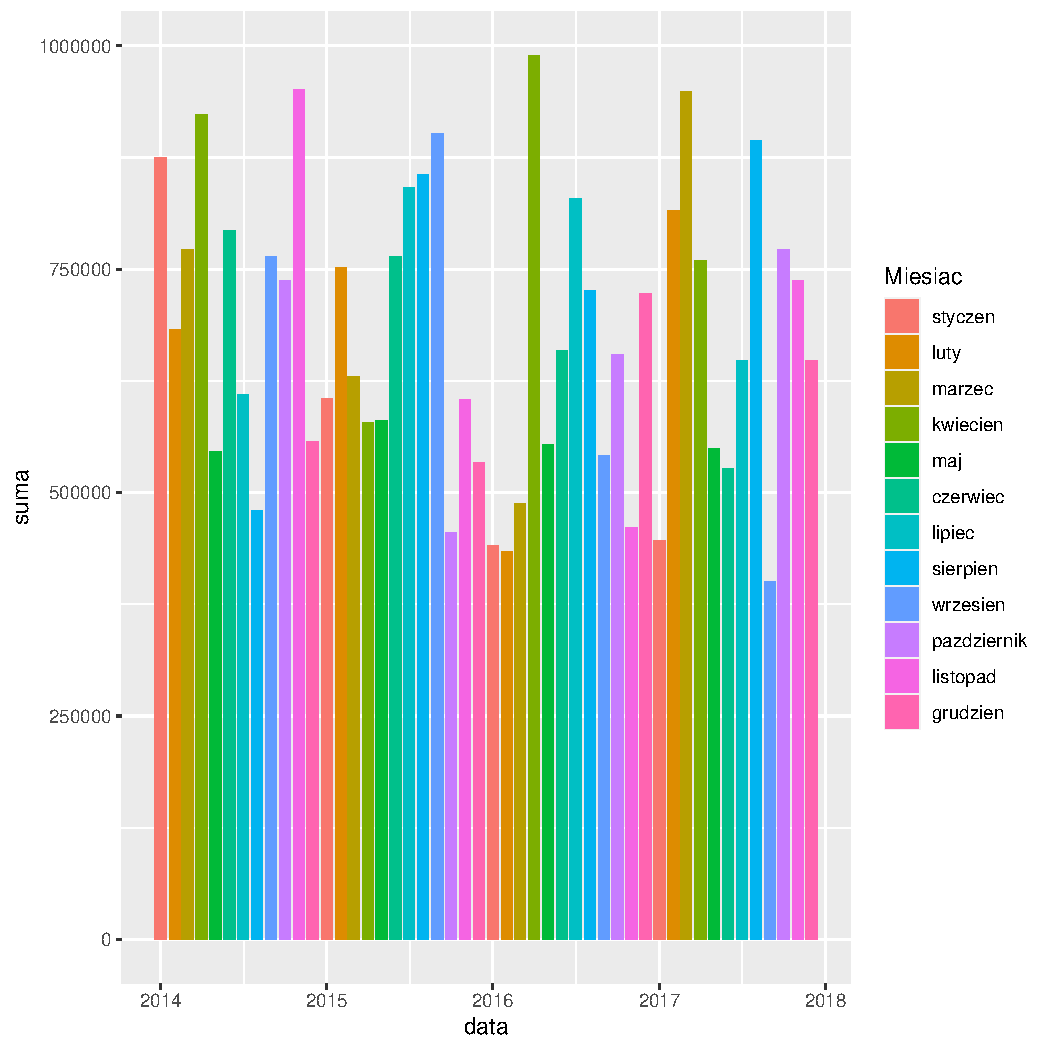
\includegraphics[width=\maxwidth]{figure/unnamed-chunk-5-1} 
\end{knitrout}


\subsection{Analiza wydatków na zakup części}

\begin{knitrout}
\definecolor{shadecolor}{rgb}{0.969, 0.969, 0.969}\color{fgcolor}
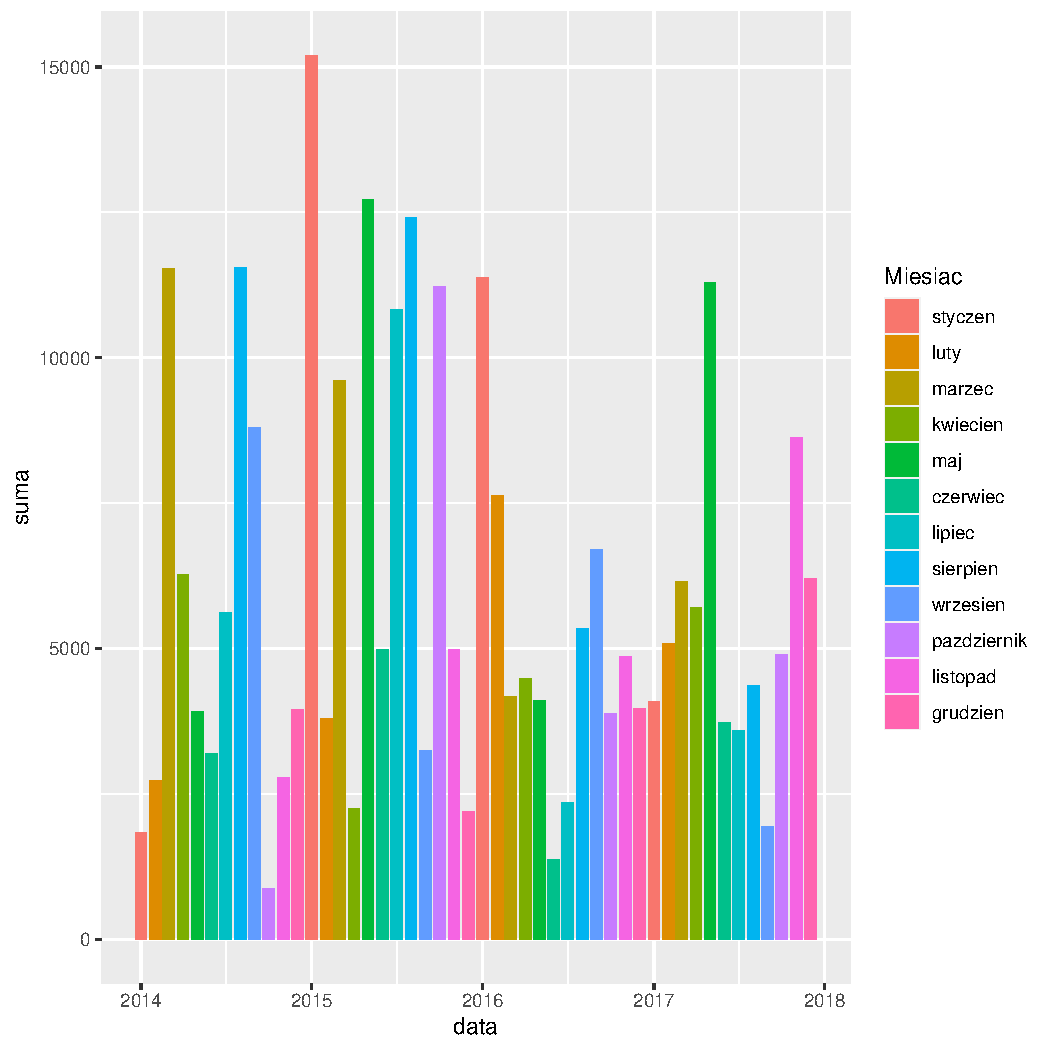
\includegraphics[width=\maxwidth]{figure/unnamed-chunk-6-1} 
\end{knitrout}

\subsection{Analiza przychodów z usług warsztatu}

Chcielibyśmy sprawdzić, jak wyglądają miesięczne przychody (lub straty) wynikające z prowadzenia warsztatu. Przez przychód za pojedyńczą usługę uważamy różnicę ceny, którą zapłacił klient i kwoty zapłaconej za części.

\begin{knitrout}
\definecolor{shadecolor}{rgb}{0.969, 0.969, 0.969}\color{fgcolor}
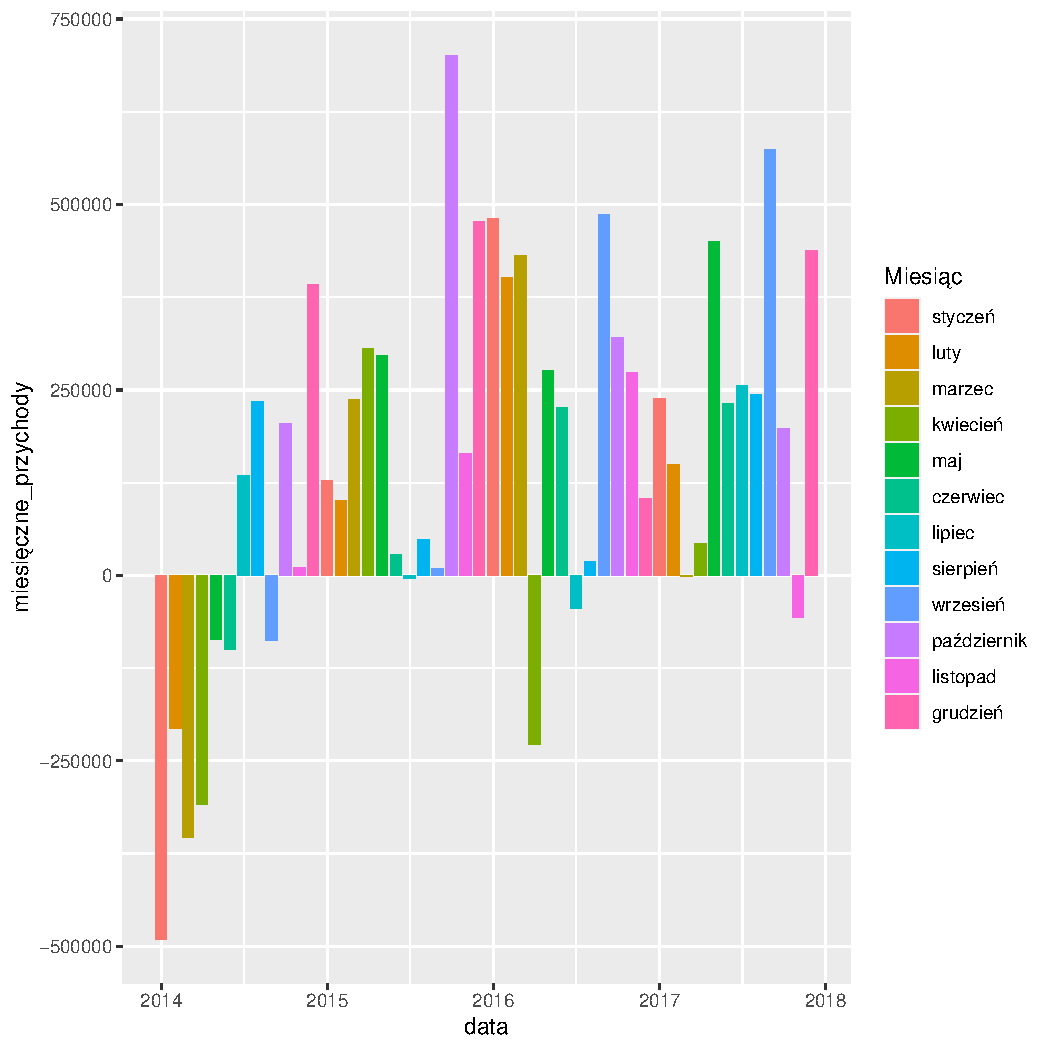
\includegraphics[width=\maxwidth]{figure/unnamed-chunk-7-1} 
\end{knitrout}

{\color{red} tAK JAK WYŻEJ}

\begin{knitrout}
\definecolor{shadecolor}{rgb}{0.969, 0.969, 0.969}\color{fgcolor}
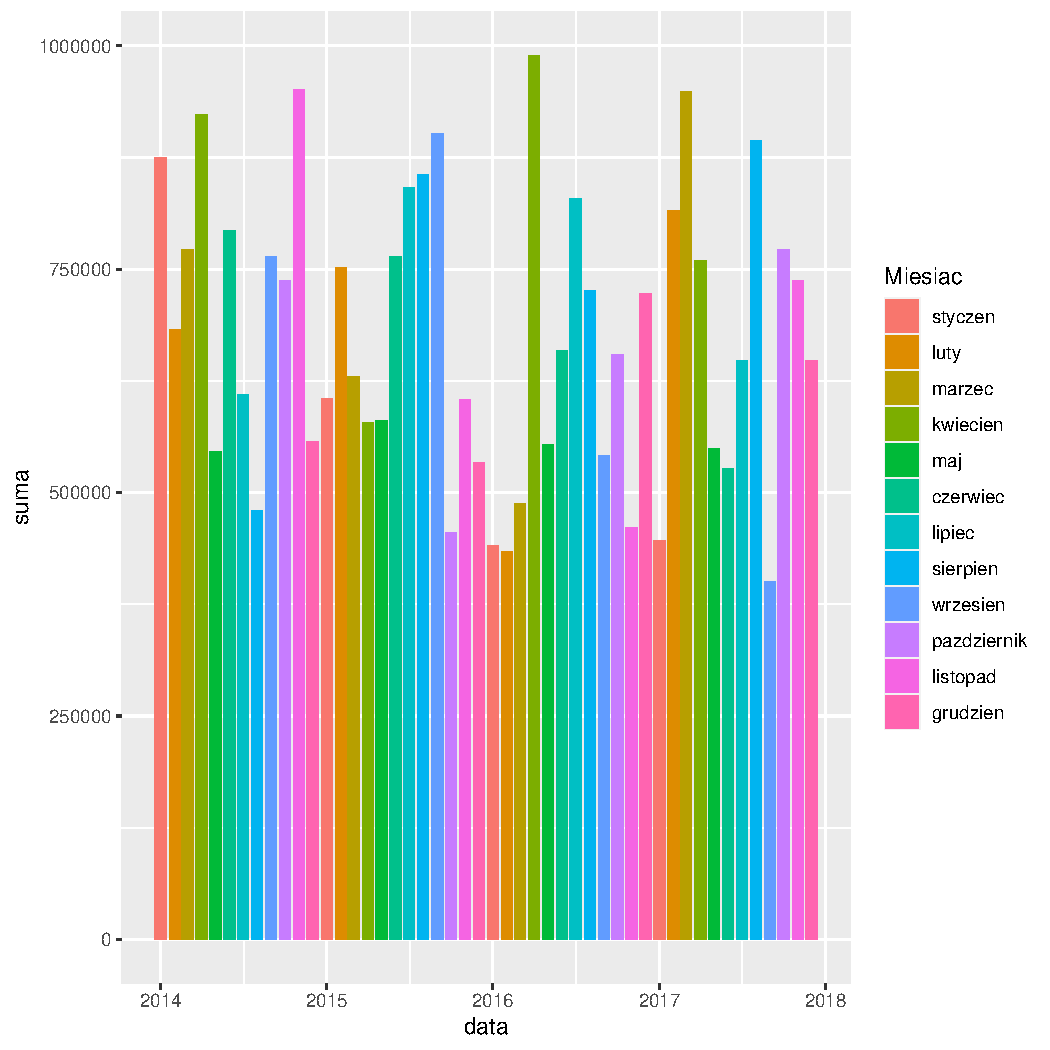
\includegraphics[width=\maxwidth]{figure/unnamed-chunk-8-1} 
\end{knitrout}

{\color{red} SAME ZYSKI, WŁASNYCH NIE LICZYMY}

\subsection{Koszty wypłat dla pracowników}

{\color{red} NA RAZIE NIE MAM}

\subsection{Samochody wpływy}

{\color{red} MOŻE BYĆ TRUDNE BO RATY}

\subsection{Razem na miesiąc}

{\color{red} JAK TO WYZEJ SIĘ UDA}


\section{Kim są najlepszy mechanik i sprzedawca w warsztacie?}

Przez czas działania warsztatu „Pimp My Wheels” osoba zarządzająca warsztatem nie była skłonna do dawania podwyżek, jednak postanowiła zlecić informatykowi by przeanalizował bazę danych i znalazł pracowników, którzy zasługują na większe wynagrodzenie. \\




Osoba, która sprzedała w firmie najbardziej wartościowe pojazdy to Janusz Kończal. Ta osoba zarobiła dla firmy 25277132.54 zł na sprzedaży pojazdów, co stanowi 112.19\% średniej kwoty zarobionej dla warsztatu przez cały okres pracy. W porównaniu, zarabiana przez tego pracownika kwota za godzinę pracy (59.50 zł) stanowi 105.03 \% średniej płacy sprzedawcy (56.65 zł). Różnica procentowa wynosi 7.16\%, czyli warsztat zdecydowanie powinien rozważyć podwyżkę dla tego pracownika, by lepiej wyróżnić jego wpływ na dochody firmy. \\

Pracownik, który sprzedał najwięcej pojazdów to ponownie Janusz Kończal. Ta osoba sprzedała aż 413 pojazdów, co stanowi 106.99\% średnich sprzedaży przypadających na pracownika. Patrząc na zarobki pracownika można zauważyć, że zarabia on za godzinę pracy (59.50 zł), czyli 105.03 \% średniej płacy sprzedawcy (56.65 zł). Między tymi dwoma wartościami wynosi 1.96\%, czyli zwiększenie stawki tego sprzedawcy nie jest niezbędne, z powodu niewielkiej różnicy. Drobna podwyżka mogłaby za to pozytywnie wpłynąć na ilość sprzedaży i motywację pracownika, 

\begin{knitrout}
\definecolor{shadecolor}{rgb}{0.969, 0.969, 0.969}\color{fgcolor}\begin{kframe}


{\ttfamily\noindent\bfseries\color{errorcolor}{\#\# Error in `[.data.frame`(najwiecej\_sprzedaży, , 5): nie wybrano kolumn}}

{\ttfamily\noindent\bfseries\color{errorcolor}{\#\# Error in round(najwiecej\_sprzedaży\$ile\_sprzedanych, 2): argument nieliczbowy przekazany do funkcji matematycznej}}

{\ttfamily\noindent\bfseries\color{errorcolor}{\#\# Error in `[.data.frame`(najwiecej\_sprzedaży, , 5): nie wybrano kolumn}}\end{kframe}
\end{knitrout}


Osoba, która zarobiła dla firmy najwięcej na naprawach to Józef Stępień. Ta osoba zarobiła dla firmy 101238.00 zł na sprzedaży pojazdów, co stanowi 121.28\% średniej kwoty zarobionej dla warsztatu przez cały okres pracy wśród mechaników. W porównaniu, zarabiana przez tego pracownika kwota za godzinę pracy (53.00 zł) stanowi 100.95 \% średniej płacy sprzedawcy (52.50 zł). Różnica procentowa wynosi 20.33\%, czyli warsztat zdecydowanie powinien rozważyć podwyżkę dla tego pracownika, by lepiej wyróżnić jego wpływ na dochody firmy. \\

Pracownik, który sprzedał najwięcej pojazdów to ponownie Janusz Kończal. Ta osoba sprzedała aż 413 pojazdów, co stanowi 106.99\% średnich sprzedaży przypadających na pracownika. Patrząc na zarobki pracownika można zauważyć, że zarabia on za godzinę pracy (59.50 zł), czyli 105.03 \% średniej płacy sprzedawcy (56.65 zł). Między tymi dwoma wartościami wynosi 1.96\%, czyli zwiększenie stawki tego sprzedawcy nie jest niezbędne, z powodu niewielkiej różnicy. Drobna podwyżka mogłaby za to pozytywnie wpłynąć na ilość sprzedaży i motywację pracownika, 


\begin{knitrout}
\definecolor{shadecolor}{rgb}{0.969, 0.969, 0.969}\color{fgcolor}\begin{kframe}
\begin{alltt}
\hlkwd{dbDisconnect}\hlstd{(con)}
\end{alltt}
\end{kframe}
\end{knitrout}
\end{document}
